\documentclass[11pt]{article}
\usepackage[textwidth=18.0cm, textheight=23.0cm, top=2.0cm]{geometry}
\usepackage{pst-all}
\usepackage{amssymb}
\usepackage{tikz}
\usepackage{underscore}\begin{document}
\pagestyle{empty}


ClassName: \underline{\textbf{Class_02.2bp-27}}
\par
BinSize: \underline{\textbf{30 × 30}}
\par
ReduceSize: \underline{\textbf{30 × 30}}
\par
TypeNum: \underline{\textbf{49}}
\par
Num: \underline{\textbf{60}}
\par
OutS: \underline{\textbf{2700}}
\par
InS: \underline{\textbf{1883}}
\par
Rate: \underline{\textbf{0.697}}
\par
UB: \underline{\textbf{3}}
\par
LB0: \underline{\textbf{3}}
\par
LB: \underline{\textbf{3}}
\par
LBWithCut: \underline{\textbf{3}}
\par
NodeCut: \underline{\textbf{0}}
\par
ExtendedNodeCnt: \underline{\textbf{1}}
\par
GenNodeCnt: \underline{\textbf{1}}
\par
PrimalNode: \underline{\textbf{0}}
\par
ColumnCount: \underline{\textbf{3}}
\par
TotalCutCount: \underline{\textbf{0}}
\par
RootCutCount: \underline{\textbf{0}}
\par
LPSolverCnt: \underline{\textbf{1}}
\par
PricingSolverCnt: \underline{\textbf{0}}
\par
BranchAndBoundNum: \underline{\textbf{1}}
\par
isOpt: \underline{\textbf{true}}
\par
TimeOnInitSolution: \underline{\textbf{0.000 s}}
\par
TimeOnPrimal: \underline{\textbf{0.000 s}}
\par
TimeOnPricing: \underline{\textbf{0.000 s}}
\par
TimeOnRmp: \underline{\textbf{0.063 s}}
\par
TotalTime: \underline{\textbf{0.125 s}}
\par
\newpage


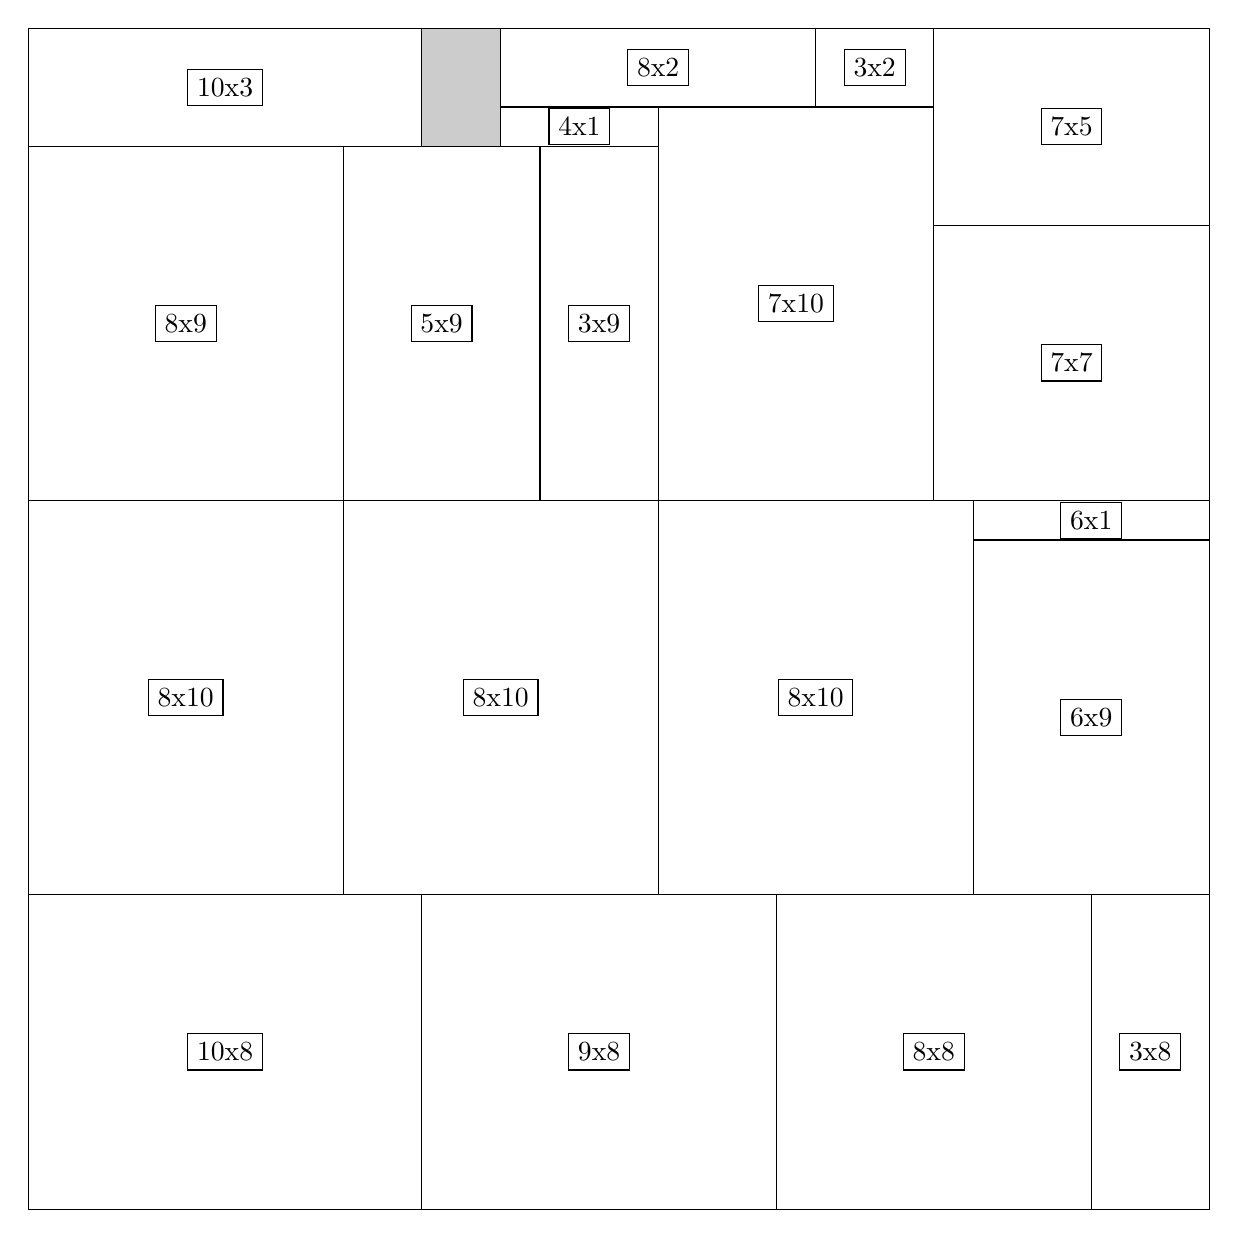
\begin{tikzpicture}[shorten >=1pt,scale=1.0,every node/.style={scale=1.0},->]
\tikzstyle{vertex}=[circle,fill=black!25,minimum size=14pt,inner sep=0pt]
\filldraw[fill=gray!40!white, draw=black] (0,0) rectangle (15.0,15.0);
\foreach \name/\x/\y/\w/\h in {10x8/0.0/0.0/5.0/4.0,8x10/0.0/4.0/4.0/5.0,8x10/4.0/4.0/4.0/5.0,8x10/8.0/4.0/4.0/5.0,9x8/5.0/0.0/4.5/4.0,8x9/0.0/9.0/4.0/4.5,7x10/8.0/9.0/3.5/5.0,8x8/9.5/0.0/4.0/4.0,6x9/12.0/4.0/3.0/4.5,7x7/11.5/9.0/3.5/3.5,5x9/4.0/9.0/2.5/4.5,7x5/11.5/12.5/3.5/2.5,10x3/0.0/13.5/5.0/1.5,3x9/6.5/9.0/1.5/4.5,3x8/13.5/0.0/1.5/4.0,8x2/6.0/14.0/4.0/1.0,6x1/12.0/8.5/3.0/0.5,3x2/10.0/14.0/1.5/1.0,4x1/6.0/13.5/2.0/0.5}
\filldraw[fill=white!40!white, draw=black] (\x,\y) rectangle node[draw] (\name) {\name} ++(\w,\h);
\end{tikzpicture}


w =10 , h =8 , x =0 , y =0 , v =80
\par
w =8 , h =10 , x =0 , y =8 , v =80
\par
w =8 , h =10 , x =8 , y =8 , v =80
\par
w =8 , h =10 , x =16 , y =8 , v =80
\par
w =9 , h =8 , x =10 , y =0 , v =72
\par
w =8 , h =9 , x =0 , y =18 , v =72
\par
w =7 , h =10 , x =16 , y =18 , v =70
\par
w =8 , h =8 , x =19 , y =0 , v =64
\par
w =6 , h =9 , x =24 , y =8 , v =54
\par
w =7 , h =7 , x =23 , y =18 , v =49
\par
w =5 , h =9 , x =8 , y =18 , v =45
\par
w =7 , h =5 , x =23 , y =25 , v =35
\par
w =10 , h =3 , x =0 , y =27 , v =30
\par
w =3 , h =9 , x =13 , y =18 , v =27
\par
w =3 , h =8 , x =27 , y =0 , v =24
\par
w =8 , h =2 , x =12 , y =28 , v =16
\par
w =6 , h =1 , x =24 , y =17 , v =6
\par
w =3 , h =2 , x =20 , y =28 , v =6
\par
w =4 , h =1 , x =12 , y =27 , v =4
\par
\newpage


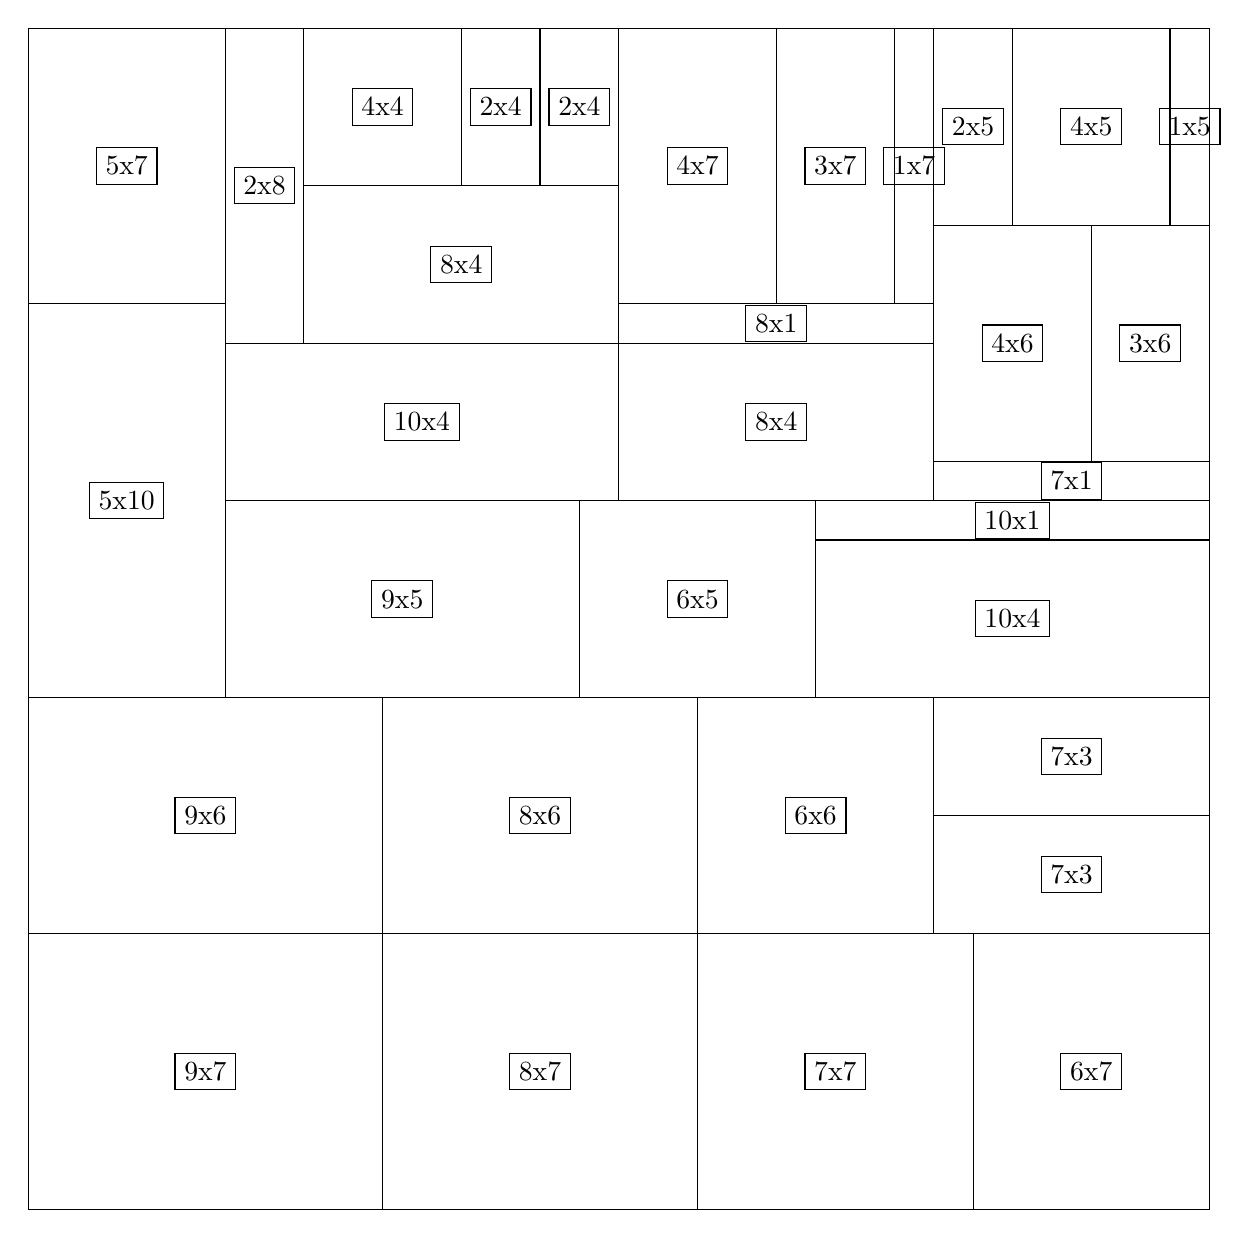
\begin{tikzpicture}[shorten >=1pt,scale=1.0,every node/.style={scale=1.0},->]
\tikzstyle{vertex}=[circle,fill=black!25,minimum size=14pt,inner sep=0pt]
\filldraw[fill=gray!40!white, draw=black] (0,0) rectangle (15.0,15.0);
\foreach \name/\x/\y/\w/\h in {9x7/0.0/0.0/4.5/3.5,8x7/4.5/0.0/4.0/3.5,9x6/0.0/3.5/4.5/3.0,5x10/0.0/6.5/2.5/5.0,7x7/8.5/0.0/3.5/3.5,8x6/4.5/3.5/4.0/3.0,9x5/2.5/6.5/4.5/2.5,6x7/12.0/0.0/3.0/3.5,10x4/10.0/6.5/5.0/2.0,10x4/2.5/9.0/5.0/2.0,6x6/8.5/3.5/3.0/3.0,5x7/0.0/11.5/2.5/3.5,8x4/7.5/9.0/4.0/2.0,8x4/3.5/11.0/4.0/2.0,6x5/7.0/6.5/3.0/2.5,4x7/7.5/11.5/2.0/3.5,4x6/11.5/9.5/2.0/3.0,7x3/11.5/3.5/3.5/1.5,7x3/11.5/5.0/3.5/1.5,3x7/9.5/11.5/1.5/3.5,2x5/11.5/12.5/1.0/2.5,3x6/13.5/9.5/1.5/3.0,4x4/3.5/13.0/2.0/2.0,2x8/2.5/11.0/1.0/4.0,10x1/10.0/8.5/5.0/0.5,4x5/12.5/12.5/2.0/2.5,8x1/7.5/11.0/4.0/0.5,2x4/5.5/13.0/1.0/2.0,2x4/6.5/13.0/1.0/2.0,7x1/11.5/9.0/3.5/0.5,1x7/11.0/11.5/0.5/3.5,1x5/14.5/12.5/0.5/2.5}
\filldraw[fill=white!40!white, draw=black] (\x,\y) rectangle node[draw] (\name) {\name} ++(\w,\h);
\end{tikzpicture}


w =9 , h =7 , x =0 , y =0 , v =63
\par
w =8 , h =7 , x =9 , y =0 , v =56
\par
w =9 , h =6 , x =0 , y =7 , v =54
\par
w =5 , h =10 , x =0 , y =13 , v =50
\par
w =7 , h =7 , x =17 , y =0 , v =49
\par
w =8 , h =6 , x =9 , y =7 , v =48
\par
w =9 , h =5 , x =5 , y =13 , v =45
\par
w =6 , h =7 , x =24 , y =0 , v =42
\par
w =10 , h =4 , x =20 , y =13 , v =40
\par
w =10 , h =4 , x =5 , y =18 , v =40
\par
w =6 , h =6 , x =17 , y =7 , v =36
\par
w =5 , h =7 , x =0 , y =23 , v =35
\par
w =8 , h =4 , x =15 , y =18 , v =32
\par
w =8 , h =4 , x =7 , y =22 , v =32
\par
w =6 , h =5 , x =14 , y =13 , v =30
\par
w =4 , h =7 , x =15 , y =23 , v =28
\par
w =4 , h =6 , x =23 , y =19 , v =24
\par
w =7 , h =3 , x =23 , y =7 , v =21
\par
w =7 , h =3 , x =23 , y =10 , v =21
\par
w =3 , h =7 , x =19 , y =23 , v =21
\par
w =2 , h =5 , x =23 , y =25 , v =10
\par
w =3 , h =6 , x =27 , y =19 , v =18
\par
w =4 , h =4 , x =7 , y =26 , v =16
\par
w =2 , h =8 , x =5 , y =22 , v =16
\par
w =10 , h =1 , x =20 , y =17 , v =10
\par
w =4 , h =5 , x =25 , y =25 , v =20
\par
w =8 , h =1 , x =15 , y =22 , v =8
\par
w =2 , h =4 , x =11 , y =26 , v =8
\par
w =2 , h =4 , x =13 , y =26 , v =8
\par
w =7 , h =1 , x =23 , y =18 , v =7
\par
w =1 , h =7 , x =22 , y =23 , v =7
\par
w =1 , h =5 , x =29 , y =25 , v =5
\par
\newpage


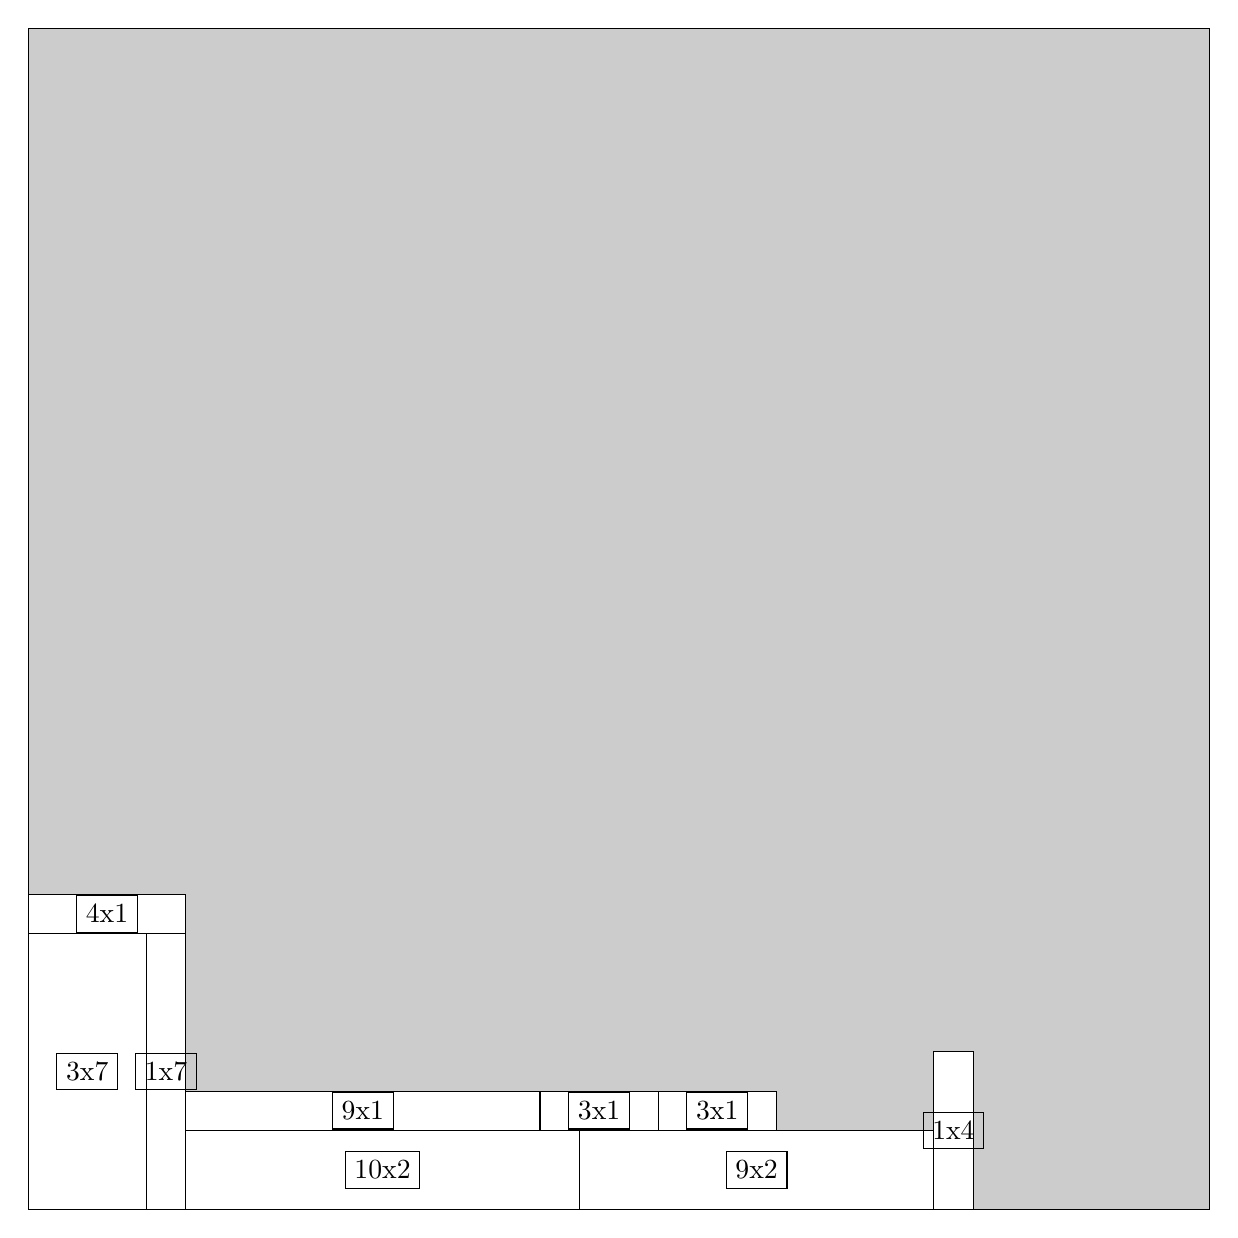
\begin{tikzpicture}[shorten >=1pt,scale=1.0,every node/.style={scale=1.0},->]
\tikzstyle{vertex}=[circle,fill=black!25,minimum size=14pt,inner sep=0pt]
\filldraw[fill=gray!40!white, draw=black] (0,0) rectangle (15.0,15.0);
\foreach \name/\x/\y/\w/\h in {3x7/0.0/0.0/1.5/3.5,10x2/2.0/0.0/5.0/1.0,9x2/7.0/0.0/4.5/1.0,9x1/2.0/1.0/4.5/0.5,1x7/1.5/0.0/0.5/3.5,4x1/0.0/3.5/2.0/0.5,1x4/11.5/0.0/0.5/2.0,3x1/6.5/1.0/1.5/0.5,3x1/8.0/1.0/1.5/0.5}
\filldraw[fill=white!40!white, draw=black] (\x,\y) rectangle node[draw] (\name) {\name} ++(\w,\h);
\end{tikzpicture}


w =3 , h =7 , x =0 , y =0 , v =21
\par
w =10 , h =2 , x =4 , y =0 , v =20
\par
w =9 , h =2 , x =14 , y =0 , v =18
\par
w =9 , h =1 , x =4 , y =2 , v =9
\par
w =1 , h =7 , x =3 , y =0 , v =7
\par
w =4 , h =1 , x =0 , y =7 , v =4
\par
w =1 , h =4 , x =23 , y =0 , v =4
\par
w =3 , h =1 , x =13 , y =2 , v =3
\par
w =3 , h =1 , x =16 , y =2 , v =3
\par
\newpage


\end{document}